\chapter{Introducción específica} % Main chapter title

\label{Chapter2}

%----------------------------------------------------------------------------------------
%	SECTION 1
%----------------------------------------------------------------------------------------

En este capítulo se introducen los protocolos de comunicación, los diversos componentes de hardware y las herramientas de software utilizadas para el desarrollo del trabajo. 

\section{Protocolos de comunicación}

\subsection{\emph{Hypertext Transfer Protocol}}

HTTP es un protocolo de la capa de aplicación \citep{WEBSITE:CAPADEAPLICACION} para la transmisión de documentos hipermedia, como HTML (del inglés \textit{HyperText Markup Language}) \citep{WEBSITE:HTML}. Fue diseñado para la comunicación entre los navegadores y servidores web, aunque se puede utilizar para otros propósitos también. 

Sigue el clásico modelo cliente-servidor \citep{WEBSITE:CLIENTESERVIDOR}, en el que un cliente establece una conexión con el servidor, realiza una petición y espera hasta que recibe una respuesta del mismo. 

Se trata de un protocolo sin estados \citep{WEBSITE:PROTOCOLOSINESTADO}, lo cual significa que el servidor no guarda información entre dos peticiones distintas. 

Aunque en la mayoría de casos se basa en una conexión del tipo TCP/IP (del inglés \textit{Transmission Control Protocol/Internet Protocol}) \citep{WEBSITE:TCPIP} y se puede usar sobre cualquier capa de transporte \citep{WEBSITE:CAPADETRANSPORTE} segura o de confianza.

Las características claves de HTTP son:
\begin{itemize}
\item Es sencillo: HTTP está pensado y desarrollado para ser leído y fácilmente interpretado por sus usuarios. Esto facilita depurar errores y reduce su curva de aprendizaje.
\item Es extensible: las cabeceras de HTTP han hecho que este protocolo sea fácil de ampliar y de experimentar con él.
\item Es un protocolo con sesiones pero sin estados.
\end{itemize}

En la figura \ref{fig:ejemploDeComunicacionEnHTTP} se presenta un ejemplo de comunicación HTTP en el que puede observarse como interactúa un cliente con el servidor.

\begin{figure}[H]
	\centering
	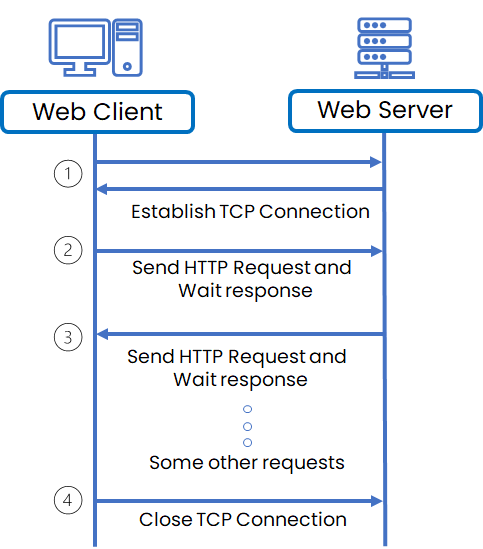
\includegraphics[width=.6\textwidth]{./Figures/Ejemplo de comunicacion en HTTP.png}
	\caption{Ejemplo de comunicacion en HTTP\protect\footnotemark.}
	\label{fig:ejemploDeComunicacionEnHTTP}
\end{figure}

\footnotetext{Imagen tomada de \newline  \url{https://www.ionos.co.uk/digitalguide/hosting/technical-matters/what-is-http/}}

La versión encriptada de HTTP se llama HTTPS (del inglés \textit{Hypertext Transfer Protocol Secure}) \citep{WEBSITE:HTTPS}. Normalmente utiliza TLS para cifrar toda la comunicación entre un cliente y un servidor. Esta conexión segura permite a los clientes intercambiar datos confidenciales de forma segura con un servidor, por ejemplo, para actividades bancarias o compras en línea.

\subsection{\emph{Message Queue Telemetry Transport}}

MQTT es un protocolo de mensajería basado en estándares o conjuntos de reglas, que se utiliza para la comunicación de un equipo a otro. 

Los sensores inteligentes, los dispositivos portátiles y otros dispositivos IoT (del inglés \textit{Internet of Things}) \citep{WEBSITE:IOT} generalmente tienen que transmitir y recibir datos a través de una red con recursos restringidos y un ancho de banda limitado. Estos dispositivos IoT utilizan MQTT para la transmisión de datos, ya que resulta fácil de implementar y puede comunicar datos IoT de manera eficiente. MQTT admite mensajería bidireccional entre dispositivos y una plataforma \textit{cloud}.

El protocolo MQTT funciona según los principios del modelo de publicación o suscripción. Sus componentes son los siguientes:
\begin{itemize}
\item Cliente: es cualquier dispositivo que ejecuta una biblioteca MQTT. Si el cliente envía mensajes, actúa como editor y si recibe mensajes, actúa como receptor.
\item Agente o \emph{broker}: es el sistema que coordina los mensajes entre los diferentes clientes. Además, se encarga de otras tareas como la autorización y autenticación de los clientes, identificar a los clientes suscritos a cada tema y el envío de sus mensajes y controlar los mensajes perdidos y las sesiones del cliente. 
\item Conexión: los clientes inician la conexión al enviar un mensaje CONECTAR al agente MQTT. El agente confirma que se ha establecido una conexión al responder con un mensaje CONNACK. Los clientes nunca se conectan entre sí, solo con el agente.
\end{itemize}

En la figura \ref{fig:ejemploDeComunicacionEnMQTT} se presenta un ejemplo de comunicación MQTT en el que puede observarse como interactúan cada uno de los componentes del protocolo.
 
\begin{figure}[H]
	\centering
	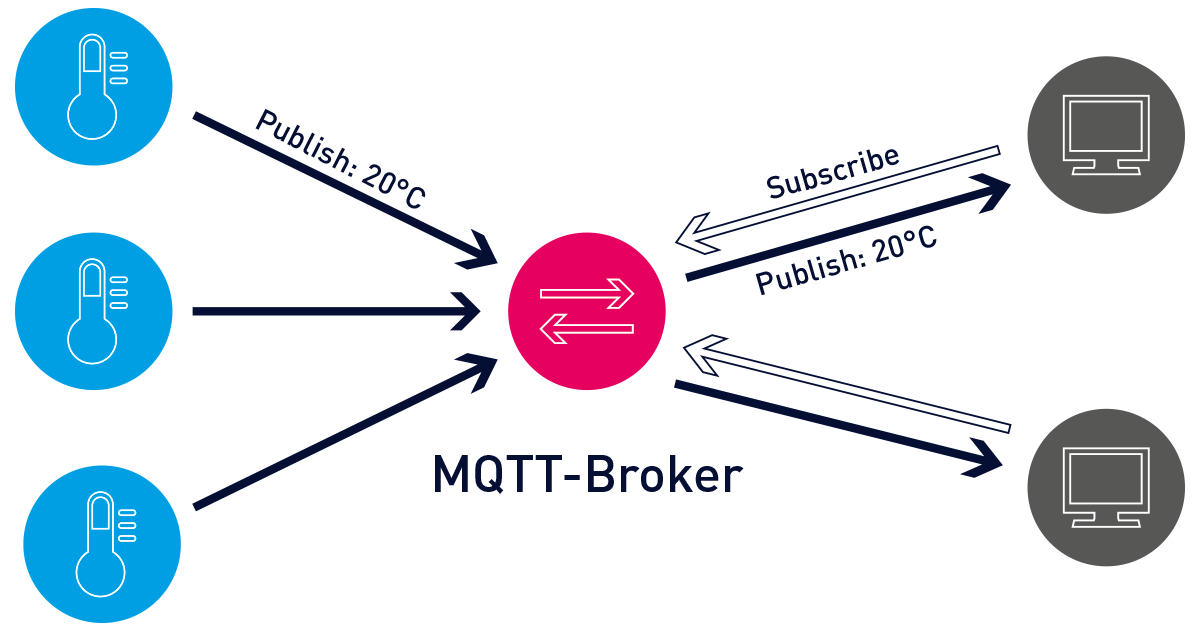
\includegraphics[width=.8\textwidth]{./Figures/Ejemplo de comunicacion en MQTT.jpg}
	\caption{Ejemplo de comunicación en MQTT\protect\footnotemark.}
	\label{fig:ejemploDeComunicacionEnMQTT}
\end{figure}

\footnotetext{Imagen tomada de \url{https://www.paessler.com/es/it-explained/mqtt}}

La comunicación MQTT utiliza el protocolo SSL para proteger los datos confidenciales que transmiten los dispositivos IoT. Puede implementar la identidad, la autenticación y la autorización entre los clientes y el agente mediante certificados SSL y contraseñas. El agente MQTT normalmente autentica a los clientes mediante sus contraseñas e identificadores únicos. En la mayoría de las implementaciones, el cliente autentica el servidor con certificados o búsquedas de DNS \citep{WEBSITE:DNS}. También puede implementar protocolos de cifrado con MQTT. 

\subsection{WebSocket}

WebSocket es una tecnología que proporciona un canal de comunicación bidireccional y full-dúplex \citep{WEBSITE:FULLDUPLEX} sobre un único \textit{socket} TCP \citep{WEBSITE:TCP}. Está diseñada para ser implementada en navegadores y servidores web, pero puede utilizarse por cualquier aplicación cliente/servidor. Además, puede utilizar SSL para las conexiones seguras y la transmisión de datos.

WebSocket utiliza un secuencia de solicitud-respuesta HTTP estándar para establecer una conexión. Una vez formada, la API WebSocket proporciona una interfaz de lectura y escritura de datos entre las partes de modo dúplex asíncrono. También proporciona una interfaz para el cierre asíncrono de la conexión desde cualquier lado.

En la figura \ref{fig:ejemploDeComunicacionEnWebSocket} se presenta un ejemplo de comunicación WebSocket, en el que puede observarse cómo interactúan el cliente y el servidor.

\begin{figure}[H]
	\centering
	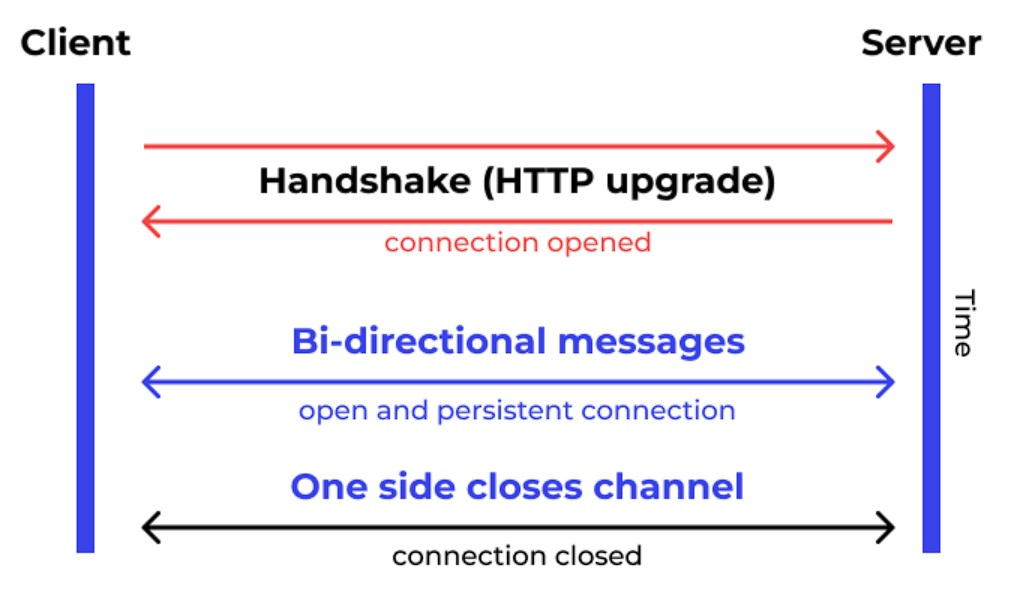
\includegraphics[width=.9\textwidth]{./Figures/Ejemplo de comunicacion en WebSocket.jpg}
	\caption{Ejemplo de comunicación en WebSocket\protect\footnotemark.}
	\label{fig:ejemploDeComunicacionEnWebSocket}
\end{figure}

\footnotetext{Imagen tomada de \newline \url{https://www.wallarm.com/what/a-simple-explanation-of-what-a-websocket-is}}

\section{Componentes de \emph{hardware}}

\subsection{Microcontrolador}

ESP32 \citep{WEBSITE:ESP32} es la denominación de una familia de chips SoC (del inglés \textit{system on a chip}) \citep{WEBSITE:SOC} de bajo coste y consumo de energía. Los integrados cuentan con tecnología Wi-Fi y Bluetooth \citep{WEBSITE:BLUETOOTH} de modo dual integrada. El ESP32 emplea un microprocesador Tensilica Xtensa LX6 en sus variantes de simple y doble núcleo e incluye interruptores de antena, balun de radiofrecuencia, amplificador de potencia, amplificador receptor de bajo ruido, filtros y módulos de administración de energía.

La elección del ESP32 se debe a los siguientes factores: 
\begin{itemize}
	\item Posee una alta disponibilidad en el mercado nacional.
	\item Tiene una alta cantidad de bibliotecas disponibles.
	\item Es económico.
	\item Es fácil de usar.
\end{itemize}

En la tabla \ref{tab:tablaBibliotecasESP32} se pueden observar las bibliotecas de terceros utilizadas en el trabajo.

\begin{table}[H]
	\centering
	\caption[Bibliotecas de terceros utilizadas]{Bibliotecas de terceros utilizadas.}
	\begin{tabular}{l c}    
		\toprule
		\textbf{Nombre} & \textbf{Descripción}\\
		\midrule
		knolleary/PubSubClient \citep{WEBSITE:PUBSUBCLIENT} & \shortstack{Permite utilizar el \\ protocolo MQTT}\\	
		adafruit/Adafruit Unified Sensor \citep{WEBSITE:ADAFRUITUNIFIEDSENSOR}& \shortstack{Dependencia para utilizar \\ el sensor DHT22}\\	
		adafruit/DHT sensor library \citep{WEBSITE:DHTSENSORLIBRARY} & \shortstack{Permite leer las mediciones \\ del sensor DHT22}\\	
		bblanchon/ArduinoJson \citep{WEBSITE:ARDUINOJSON} & Permite utilizar JSON\\	
		phoenix1747/MQ135 \citep{WEBSITE:MQ135LIBRARY} & \shortstack{Permite leer las mediciones \\ del sensor MQ135}\\	
		claws/BH1750 \citep{WEBSITE:BH1750LIBRARY} & \shortstack{Permite leer las mediciones \\ del sensor Bh1750}\\	
		milesburton/DallasTemperature \citep{WEBSITE:ARDUINOTEMPERATURECONTROLLIBRARY} & \shortstack{Permite leer las mediciones \\ del sensor DS18B20}\\	
		\bottomrule
		\hline 
	\end{tabular}
	\label{tab:tablaBibliotecasESP32}
\end{table}

\subsection{Sensor digital de temperatura y humedad}

El módulo DHT22 \citep{WEBSITE:DHT22} es un sensor digital de temperatura y humedad relativa. Integra un sensor capacitivo de humedad y un termistor \citep{WEBSITE:TERMISTOR} para medir el aire circundante y entrega la información mediante una señal digital en el pin de datos. 

Es utilizado principalmente en aplicaciones de control automático de temperatura, aire acondicionado y monitoreo ambiental en agricultura. La mayor desventaja del sensor es que sólo se puede obtener nuevos datos cada 2 segundos. 

La fotografía del sensor DHT22 se presenta en la figura \ref{fig:fotografiaDHT22}.

\begin{figure}[H]
	\centering
	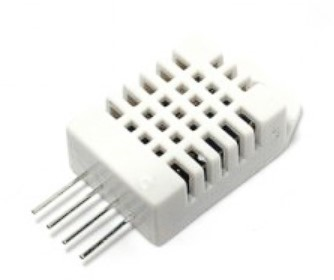
\includegraphics[width=.4\textwidth]{./Figures/DHT22.jpg}
	\caption{Fotografía del sensor DHT22\protect\footnotemark.}
	\label{fig:fotografiaDHT22}
\end{figure}

\footnotetext{Imagen tomada de \newline \url{https://www.openhacks.com/page/productos/id/84/title/Sensor-de-Humedad-y-Temperatura-DHT22}}

La elección del sensor DHT22 es debida a su mejor resolución y precisión frente a otros sensores, por ejemplo el DHT11 \citep{WEBSITE:DHT11}.


\subsection{Sensor de intensidad de luz}

El módulo Bh1750 \citep{WEBSITE:BH1750} es un sensor de intensidad de luz que esta compuesto por un conversor A/D (del inglés \textit{Analog to Digital}) \citep{WEBSITE:CONVERSORAD} de 16 bits. La principal ventaja del sensor es que brinda la intensidad luminosa en unidades de Lux.

La fotografía del sensor Bh1750 se presenta en la figura \ref{fig:fotografiaBh1750}.

\begin{figure}[H]
	\centering
	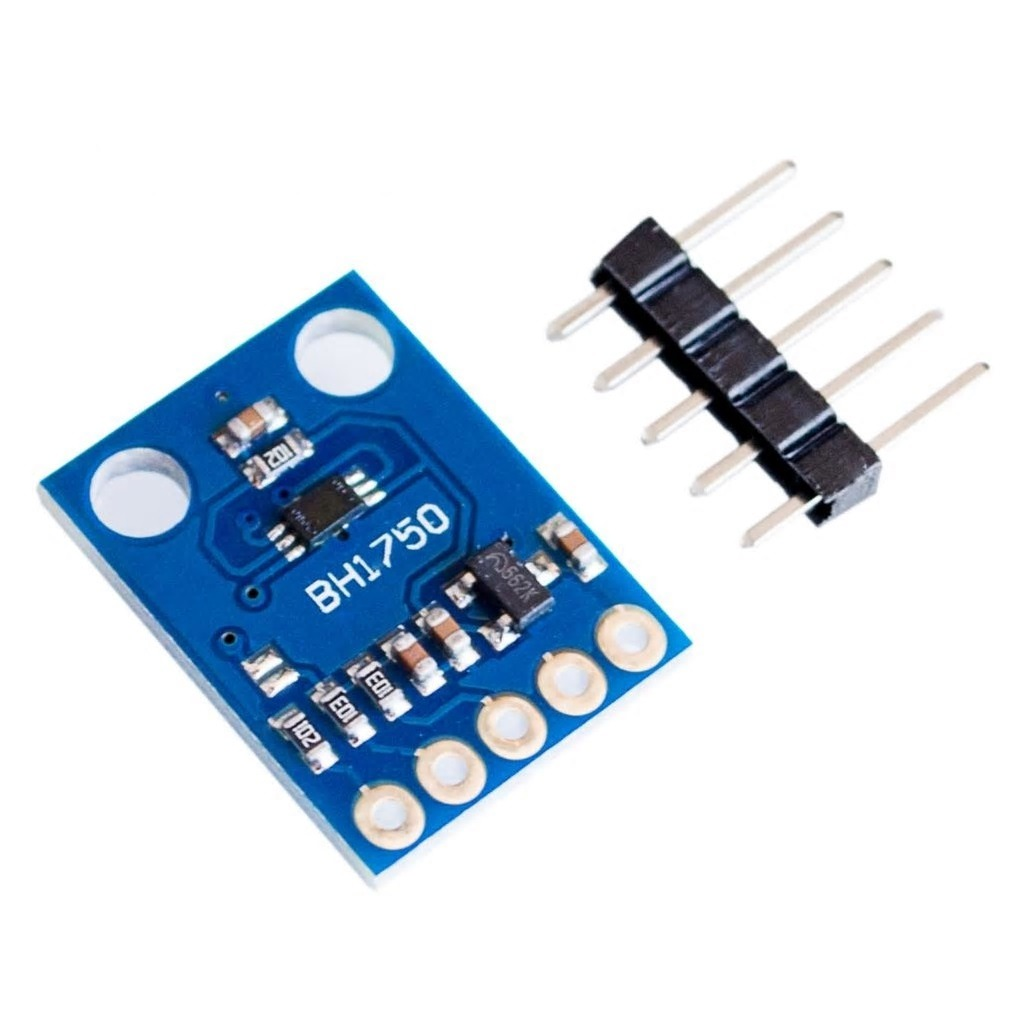
\includegraphics[width=.4\textwidth]{./Figures/Bh1750.jpg}
	\caption{Fotografía del sensor Bh1750\protect\footnotemark.}
	\label{fig:fotografiaBh1750}
\end{figure}

\footnotetext{Imagen tomada de \newline \url{https://candy-ho.com/producto/modulo-sensor-digital-luz-ambiente-lux-bh1750-arduino/}}

La elección del sensor Bh1750 es debida a su alta precisión y bajo costo en el mercado nacional. Otro factor importante en la decisión fue el poder brindar la intensidad de luz en Lux, sin necesidad de hacer alguna conversión.

\subsection{Sensor de calidad del aire}

El módulo MQ135 \citep{WEBSITE:MQ135} es un sensor de calidad del aire con alta sensibilidad al Amoníaco (NH3), óxidos de nitrógeno (NOx), alcohol, sulfuros, benceno (C6H6), CO2, humo y otros gases nocivos. Posee una salida analógica para indicar la concentración de gas en el ambiente y una digital que baja a 0 cuando la concentración de gas supera un nivel prefijado.

La fotografía del sensor MQ135 se presenta en la figura \ref{fig:fotografiaMQ135}.

\begin{figure}[H]
	\centering
	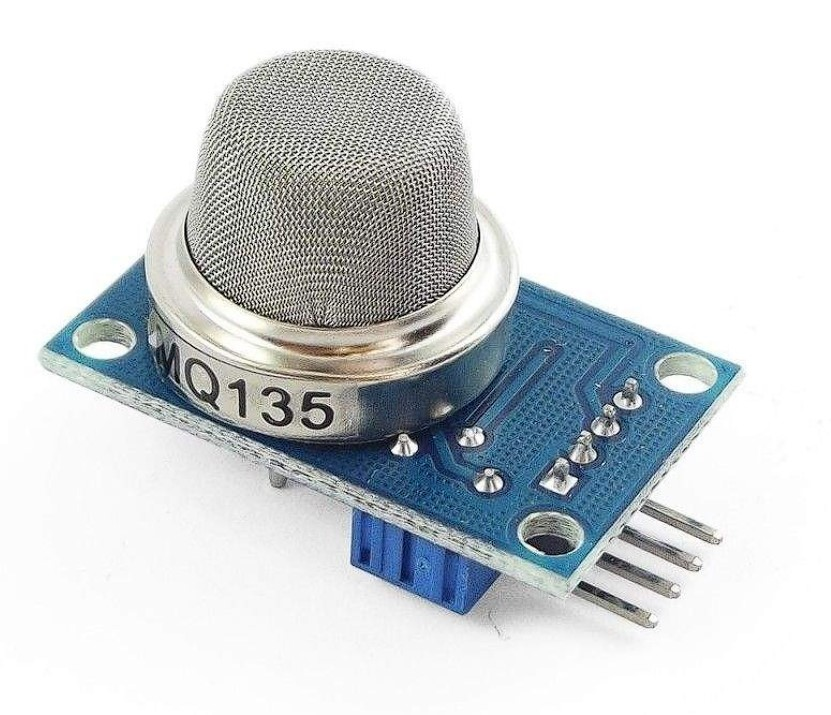
\includegraphics[width=.4\textwidth]{./Figures/MQ135.jpg}
	\caption{Fotografía del sensor MQ135\protect\footnotemark.}
	\label{fig:fotografiaMQ135}
\end{figure}

\footnotetext{Imagen tomada de \newline \url{https://www.micro-log.com/sensores-modulos-y-shields/3521-sensor-de-calidad-del-aire.html}}

La elección del sensor MQ135 es debida a su bajo costo y a la baja oferta de sensores similares en el mercado nacional.

\subsection{Sensor de flujo}

El módulo YF-S201B \citep{WEBSITE:YF-S201B} es un sensor de flujo que se utiliza para la medición de caudal o gasto volumétrico de un fluido en tuberías de 1/2” de diámetro.

Este sensor consiste en un cuerpo de válvula de plástico, un rotor y un sensor de efecto Hall \citep{WEBSITE:EFECTOHALL}. El rotor gira cuando el agua/líquido fluye a través de la válvula y su velocidad es directamente proporcional a la velocidad de flujo. El sensor de efecto Hall proporciona un impulso eléctrico con cada revolución del rotor. Este módulo sensor de flujo de agua puede ser fácilmente conectado con microcontroladores.

La fotografía del sensor YF-S201B se presenta en la figura \ref{fig:fotografiaYF-S201B}.

\begin{figure}[H]
	\centering
	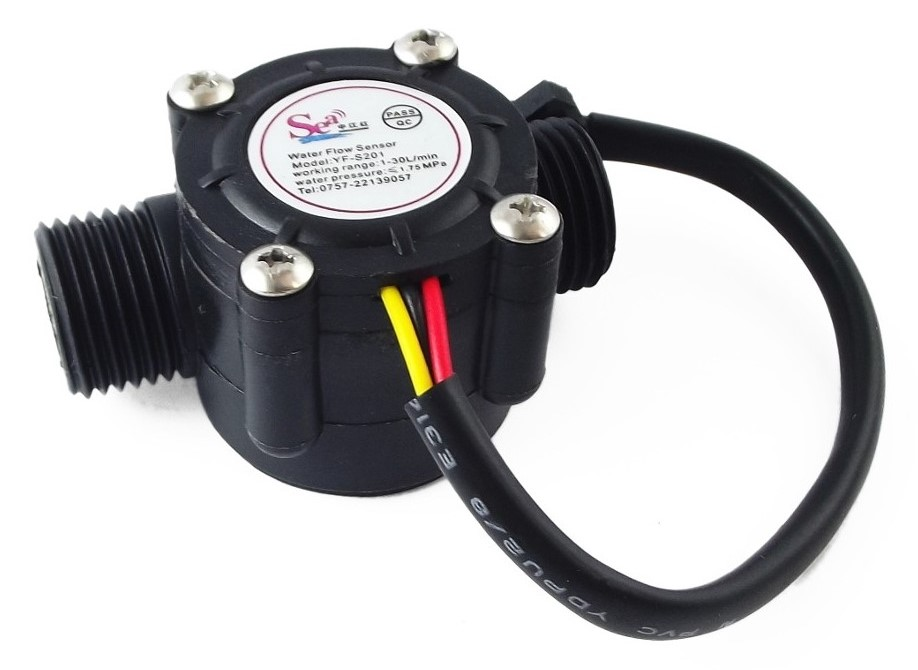
\includegraphics[width=.5\textwidth]{./Figures/YF-S201B.jpg}
	\caption{Fotografía del sensor YF-S201B\protect\footnotemark.}
	\label{fig:fotografiaYF-S201B}
\end{figure}

\footnotetext{Imagen tomada de \newline \url{https://naylampmechatronics.com/sensores-liquido/108-sensor-de-flujo-de-agua-12-yf-s201.html}}

La elección del sensor YF-S201B es debida a su bajo costo en el mercado nacional. Otros factores influyentes en la decisión fueron el bajo consumo y su facilidad de uso respecto a otros sensores similares.

\subsection{Sensor digital de temperatura para líquidos}

El módulo DS18B20 \citep{WEBSITE:DS18B20} sumergible es un sensor digital de temperatura que utiliza el protocolo 1-Wire \citep{WEBSITE:1WIRE} para comunicarse, el cual necesita solo un pin de datos y permite conectar más de un sensor en el mismo bus. La temperatura de funcionamiento es desde los -55 °C hasta los 125 °C y con una resolución programable desde 9 hasta 12 bits.

La fotografía del sensor DS18B20 sumergible se presenta en la figura \ref{fig:fotografiaDS18B20}.

\begin{figure}[H]
	\centering
	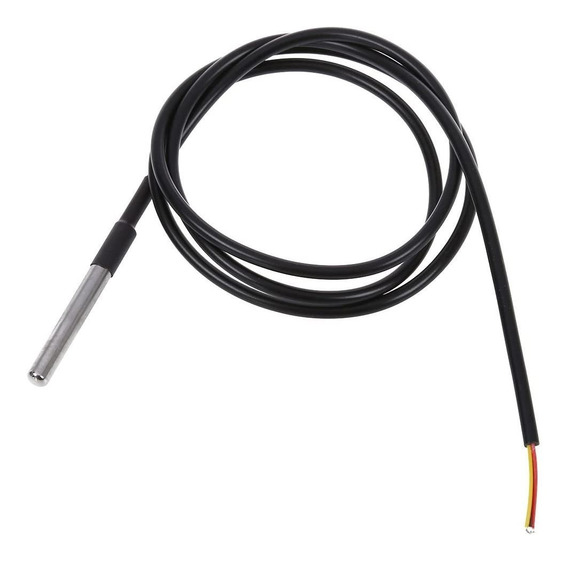
\includegraphics[width=.5\textwidth]{./Figures/DS18B20.jpg}
	\caption{Fotografía del sensor DS18B20 sumergible\protect\footnotemark.}
	\label{fig:fotografiaDS18B20}
\end{figure}

\footnotetext{Imagen tomada de \url{https://www.hobbytronica.com.ar/mla-903024959-ds18b20}}

La elección del sensor DS18B20 es debida a su facilidad de uso y amplio rango de medición.

\subsection{Módulo de \emph{relay}}

El \textit{relay} es un interruptor eléctrico para controlar el flujo de corriente. Puede estar cerrado o abierto con lo que permite o impide la circulación respectivamente.

La fotografía del módulo de \emph{relay} se presenta en la figura \ref{fig:fotografiaRelay}.

\begin{figure}[H]
	\centering
	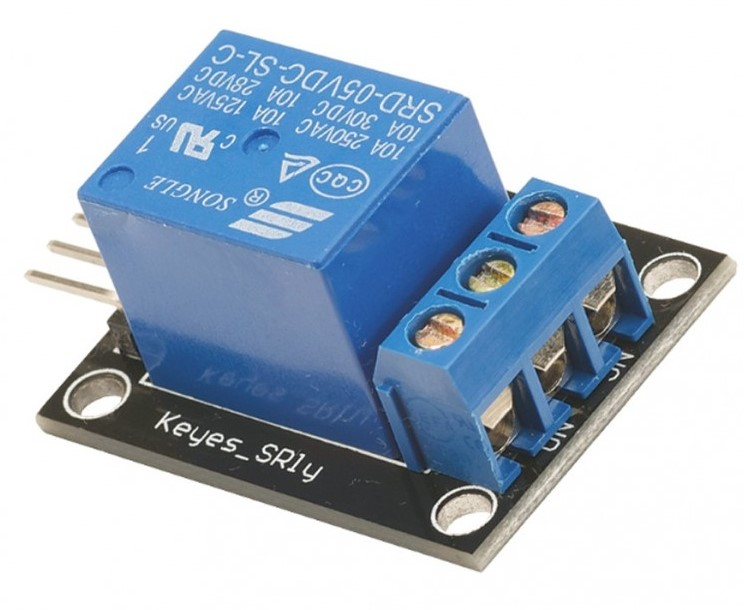
\includegraphics[width=.4\textwidth]{./Figures/Relay.jpg}
	\caption{Fotografía del módulo de \emph{relay}\protect\footnotemark.}
	\label{fig:fotografiaRelay}
\end{figure}

\footnotetext{Imagen tomada de \url{https://candy-ho.com/producto/modulo-rele-5v}}

La elección de incorporar un módulo de \emph{relay} es debida a que se quiere ofrecer al usuario del sistema un mecanismo para accionar dispositivos externos.

\section{Herramientas de \emph{software}}

\subsection{\textit{Progressive Web Apps}}

Las PWA (del inglés \textit{Progressive Web Apps}) \citep{WEBSITE:PWA} son aplicaciones web que utilizan APIs y funciones emergentes del navegador web junto a una estrategia tradicional de mejora progresiva para ofrecer una aplicación nativa. 

Para poder llamar PWA a una aplicación web, debe tener las siguientes características: uso de HTTPS, uno o más \emph{service workers} \citep{WEBSITE:SERVICEWORKERS} y un archivo de manifiesto \citep{WEBSITE:MANIFEST}.

Mediante los \emph{service workers} y otras tecnologías, las PWA pueden seguir ejecutándose en segundo plano sin tener que vivir dentro del navegador. Además, pueden instalarse en celulares y computadoras.

En la tabla \ref{tab:tablaComparacionAplicaciones} se puede observar una comparación entre aplicaciones nativas, aplicaciones web y PWA.

\begin{table}[h]
	\centering
	\caption[Comparación entre distintos tipos de aplicaciones]{Comparación entre distintos tipos de aplicaciones.}
	\begin{tabular}{l c c c}    
		\toprule
		\textbf{Descripción} & \textbf{Web} & \textbf{Nativa} & \textbf{PWA}\\
		\midrule
		Instalable & No & Sí & Sí \\	
		Multiplataforma & Sí & No & Sí \\	
		Notificaciones \emph{push} & No & Sí & Sí \\	
		Uso sin Internet & No & Sí & Sí \\	
		Diseño \emph{responsive} \citep{WEBSITE:RESPONSIVE} & Sí & Sí & Sí \\	
		Acceso al GPS & No & Sí & Sí \\
		\bottomrule
		\hline
	\end{tabular}
	\label{tab:tablaComparacionAplicaciones}
\end{table}

\subsection{\emph{Framework} del \emph{frontend}}

Angular \citep{WEBSITE:ANGULAR} es un \emph{framework} \citep{WEBSITE:FRAMEWORK} para aplicaciones web desarrollado en TypeScript \citep{WEBSITE:TYPESCRIPT}. Es de código abierto y mantenido por Google y se utiliza para crear y mantener aplicaciones web de una sola página \citep{WEBSITE:SPA}. Su objetivo es aumentar las aplicaciones basadas en navegador con capacidad de MVC (del inglés \textit{Model-View-Controller}) \citep{WEBSITE:MVC}, en un esfuerzo para hacer que el desarrollo y las pruebas sean más fáciles.

La biblioteca lee el HTML que contiene atributos de las etiquetas personalizadas adicionales, entonces obedece a las directivas de los atributos personalizados y une las piezas de entrada o salida de la página a un modelo representado por las variables estándar de JavaScript \citep{WEBSITE:JAVASCRIPT}.

Angular se basa en clases tipo componente, cuyas propiedades son las usadas para hacer el \emph{binding} de los datos. Dichas clases tienen propiedades y métodos.

La elección de Angular se debe a los siguientes factores: 
\begin{itemize}
	\item Posee alta escalabilidad.
	\item Al ser un \emph{framework} contiene muchas funcionalidades incorporadas, por ejemplo el manejo de rutas.
	\item Es fácil de adaptar a PWA.
	\item Tiene una documentación detallada.
	\item Posee una amplia variedad de bibliotecas disponibles.
	\item Tiene una comunidad activa.
\end{itemize}

En la tabla \ref{tab:tablaBibliotecasAngular} se pueden observar las bibliotecas de terceros utilizadas en la solución de Angular.

\begin{table}[h]
	\centering
	\caption[Bibliotecas de terceros utilizadas]{Bibliotecas de terceros utilizadas.}
	\begin{tabular}{l c c}    
		\toprule
		\textbf{Nombre} & \textbf{Descripción}\\
		\midrule
		@angular/material \citep{WEBSITE:ANGULARMATERIALLIBRARY} & Permite utilizar Material Design \citep{WEBSITE:ANGULARMATERIAL} \\	
		@swimlane/ngx-charts \citep{WEBSITE:NGXCHARTS} & Permite utilizar gráficos D3.js \citep{WEBSITE:D3JS} \\	
		socket.io-client \citep{WEBSITE:SOCKETIOCLIENT} & Permite utilizar Socket.IO \citep{WEBSITE:SOCKETIO} \\	
		ngx-cookieconsent \citep{WEBSITE:NGXCOOKIECONSENT} & \shortstack{Permite generar una alerta \\ del uso de cookies \citep{WEBSITE:COOKIES}} \\	
		ngx-countup \citep{WEBSITE:NGXCOUNTUP}& Permite generar animaciones numéricas \\	
		lite-server \citep{WEBSITE:LITESERVER}& \shortstack{Permite emular un despliegue \\ en un entorno local} \\	
		compression \citep{WEBSITE:COMPRESSIONLBIRARY} & Permite habilitar g-zip \citep{WEBSITE:GZIP} al usar lite-server \\	
		\bottomrule
		\hline
	\end{tabular}
	\label{tab:tablaBibliotecasAngular}
\end{table}

\subsection{Entorno en tiempo de ejecución del \emph{backend}}

Node.js \citep{WEBSITE:NODEJS} es un entorno de código abierto multiplataforma que ejecuta código JavaScript fuera de un navegador. Fue creado con el enfoque de ser útil en la creación de programas de red altamente escalables, como por ejemplo, servidores web.

La elección de Node.js se debe a los siguientes factores: 
\begin{itemize}
	\item Tiene la capacidad para manejar aplicaciones de alta concurrencia.
	\item Tiene la capacidad para escalar horizontalmente.
	\item Posee una amplia variedad de bibliotecas y paquetes disponibles.
	\item Brinda la posibilidad de usar TypeScript, tanto en el cliente como en el servidor.
	\item Tiene buen rendimiento.
	\item Tiene una comunidad activa.
\end{itemize}

En la tabla \ref{tab:tablaBibliotecasNodejs} se pueden observar las bibliotecas de terceros utilizadas en la solución de Node.js.

\begin{table}[H]
	\centering
	\caption[Bibliotecas de terceros utilizadas]{Bibliotecas de terceros utilizadas.}
	\begin{tabular}{l c c}    
		\toprule
		\textbf{Nombre} & \textbf{Descripción}\\
		\midrule
		bcryptjs \citep{WEBSITE:BCRYPTJS} & \shortstack{Permite realizar encriptaciones \citep{WEBSITE:ENCRIPTACION} \\ de contraseñas}\\	
		aedes \citep{WEBSITE:AEDES} & Permite generar un \emph{broker} MQTT \\	
		compression \citep{WEBSITE:COMPRESSIONLBIRARY} & Permite habilitar g-zip\\	
		cors \citep{WEBSITE:CORSLIBRARY} & Permite habilitar CORS \citep{WEBSITE:CORS} \\	
		dotenv \citep{WEBSITE:DOTENV} & \shortstack{Permite utilizar variables \\  de entorno \citep{WEBSITE:VARIABLESDEENTORNO}} \\	
		express \citep{WEBSITE:EXPRESSLIBRARY} & \shortstack{Permite utilizar el \\ \emph{framework} Express \citep{WEBSITE:EXPRESSJS}} \\	
		express-rate-limit \citep{WEBSITE:EXPRESSRATELIMIT} & \shortstack{Permite limitar la cantidad de \\ \textit{requests} permitidas} \\	
		jsonwebtoken \citep{WEBSITE:JSONWEBTOKENLIBRARY} & \shortstack{Permite utilizar \\ \emph{JSON Web Tokens} \citep{WEBSITE:JWT}} \\	
		mongoose \citep{WEBSITE:MONGOOSELIBRARY} & \shortstack{Permite utilizar el ORM \citep{WEBSITE:ORM} \\ mongoose \citep{WEBSITE:MONGOOSEJS}} \\	
		node-cron \citep{WEBSITE:NODECRON} & Permite programar tareas \\	
		nodemailer \citep{WEBSITE:NODEMAILER} & Permite enviar \textit{emails} \\	
		nodemailer-express-handlebars \citep{WEBSITE:NODEMAILEREXPRESSHANDLEBARS}& \shortstack{Permite agregar código \\ HTML a los \textit{emails}} \\	
		web-push \citep{WEBSITE:WEBPUSH} & Permite enviar notificaciones \emph{push}\\
		typescript \citep{WEBSITE:TYPESCRIPTLIBRARY} & Permite utilizar el lenguaje TypeScript \\
		nodemon \citep{WEBSITE:NODEMON} & \shortstack{Permite resetear automáticamente \\ el servidor si el código cambia} \\	
		supertest \citep{WEBSITE:SUPERTEST} & Permite probar servicios HTTP \\
		jest \citep{WEBSITE:JESTLIBRARY} & Permite el uso del \emph{framework} Jest \\
		ts-jest \citep{WEBSITE:TSJEST}& \shortstack{Permite usar TypeScript con \\ el \emph{framework} Jest} \\
		\bottomrule
		\hline
	\end{tabular}
	\label{tab:tablaBibliotecasNodejs}
\end{table}

\subsection{Base de datos}

MongoDB \citep{WEBSITE:MONGODB} es un sistema de base de datos NoSQL (del inglés \textit{Not Only Structured Query Language})\citep{WEBSITE:NOSQL}, orientado a documentos \citep{WEBSITE:BASEDEDATOSDOCUMENTAL} y de código abierto.

En lugar de guardar los datos en tablas, tal y como se hace en las bases de datos relacionales \citep{WEBSITE:BASEDEDATOSRELACIONAL}, MongoDB guarda estructuras de datos BSON (del inglés \textit{Binary JavaScript Object Notation}) \citep{WEBSITE:BSON} con un esquema dinámico, haciendo que la integración de los datos en ciertas aplicaciones sea más fácil y rápida. 

En la figura \ref{fig:ejemploDeModeladoDeDatosEnMongoDB} se presenta un ejemplo de modelado de datos en MongoDB, en el que puede observarse el formato de un documento BSON.

\begin{figure}[H]
	\centering
	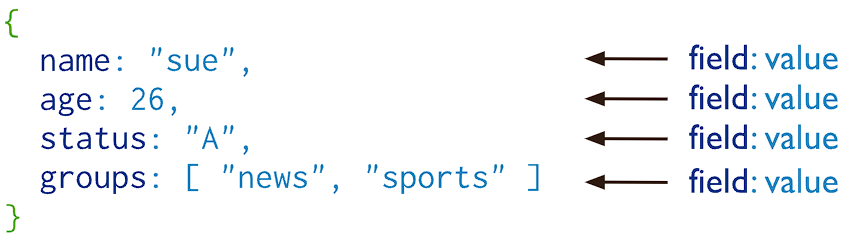
\includegraphics[width=.8\textwidth]{./Figures/Ejemplo de modelado de datos en MongoDB.png}
	\caption{Ejemplo de modelado de datos en MongoDB \protect\footnotemark.}
	\label{fig:ejemploDeModeladoDeDatosEnMongoDB}
\end{figure}

\footnotetext{Imagen tomada de \url{https://www.mongodb.com/docs/manual/core/document/}}

La elección de MongoDB se debe a los siguientes factores: 
\begin{itemize}
	\item Posee alta escalabilidad horizontal.
	\item Es altamente flexible en el modelo de datos.
	\item Tiene buen rendimiento.
	\item Es fácil de integrar con otras tecnologías.
	\item Tiene una comunidad activa.
\end{itemize}

\subsection{\emph{Framework} de pruebas del \emph{frontend}}

Jasmine \citep{WEBSITE:JASMINE} es un marco de pruebas de JavaScript diseñado para facilitar el desarrollo de pruebas automatizadas para aplicaciones web y aplicaciones escritas en JavaScript. Jasmine se basa en el patrón de pruebas BDD (del inglés \textit{Behavior-Driven Development}) \citep{WEBSITE:BDD} y se utiliza comúnmente para aplicaciones escritas en Angular.

Jasmine proporciona un conjunto de funciones y sintaxis para escribir pruebas que sean fáciles de leer y comprender.

La elección de Jasmine es debida a su integración incluida en Angular y a su velocidad de ejecución.

\subsection{\emph{Framework} de pruebas del \emph{backend}}

Jest \citep{WEBSITE:JESTJS} es un marco de pruebas de JavaScript desarrollado por Facebook. Al igual que Jasmine, Jest se utiliza para escribir y ejecutar pruebas automatizadas para aplicaciones web y aplicaciones escritas en JavaScript. Jest también se basa en el patrón de pruebas BDD y proporciona una sintaxis de prueba intuitiva y fácil de leer.

Jest se destaca por su velocidad de ejecución, que se debe en parte a su capacidad de realizar pruebas en paralelo y al uso de técnicas avanzadas de procesamiento en segundo plano. Jest también viene con una variedad de herramientas y utilidades para ayudar a los desarrolladores a escribir y ejecutar pruebas, incluyendo funciones de aserción para comparar valores, funciones  para configurar y limpiar el estado de las pruebas y utilidades para simular el comportamiento de objetos y funciones.

Además, Jest tiene una serie de características únicas, como la capacidad de realizar instantáneas \citep{WEBSITE:COPIAINSTANTANEA} de componentes de la interfaz de usuario y comprobarlos automáticamente para detectar cambios, así como la capacidad de integrarse con herramientas populares de automatización de tareas como Webpack \citep{WEBSITE:WEBPACK} y Babel \citep{WEBSITE:BABEL}. 

La elección de Jest se debe a los siguientes factores: 
\begin{itemize}
	\item Es fácil de usar.
	\item Es fácil de integrar con Node.js.
	\item Es rápido y eficiente.
	\item Tiene una función integrada para realizar cobertura de código.
	\item Tiene una gran comunidad activa.
\end{itemize}

\subsection{\emph{Software} de auditorías del \emph{frontend}}

Lighthouse \citep{WEBSITE:LIGHTHOUSE} es una herramienta automatizada de código abierto para mejorar la calidad de las páginas web. Se puede ejecutar contra cualquier página web pública o que requiera autenticación. Además, tiene auditorías de rendimiento, accesibilidad, PWA, mejores prácticas y SEO (del inglés \textit{Search Engine Optimization}).

En la figura \ref{fig:ejemploDeAuditoriaLighthouse} se presenta un ejemplo de una auditoría realizada con Lighthouse, en el que puede observarse las diferentes áreas que se evalúan.

\begin{figure}[H]
	\centering
	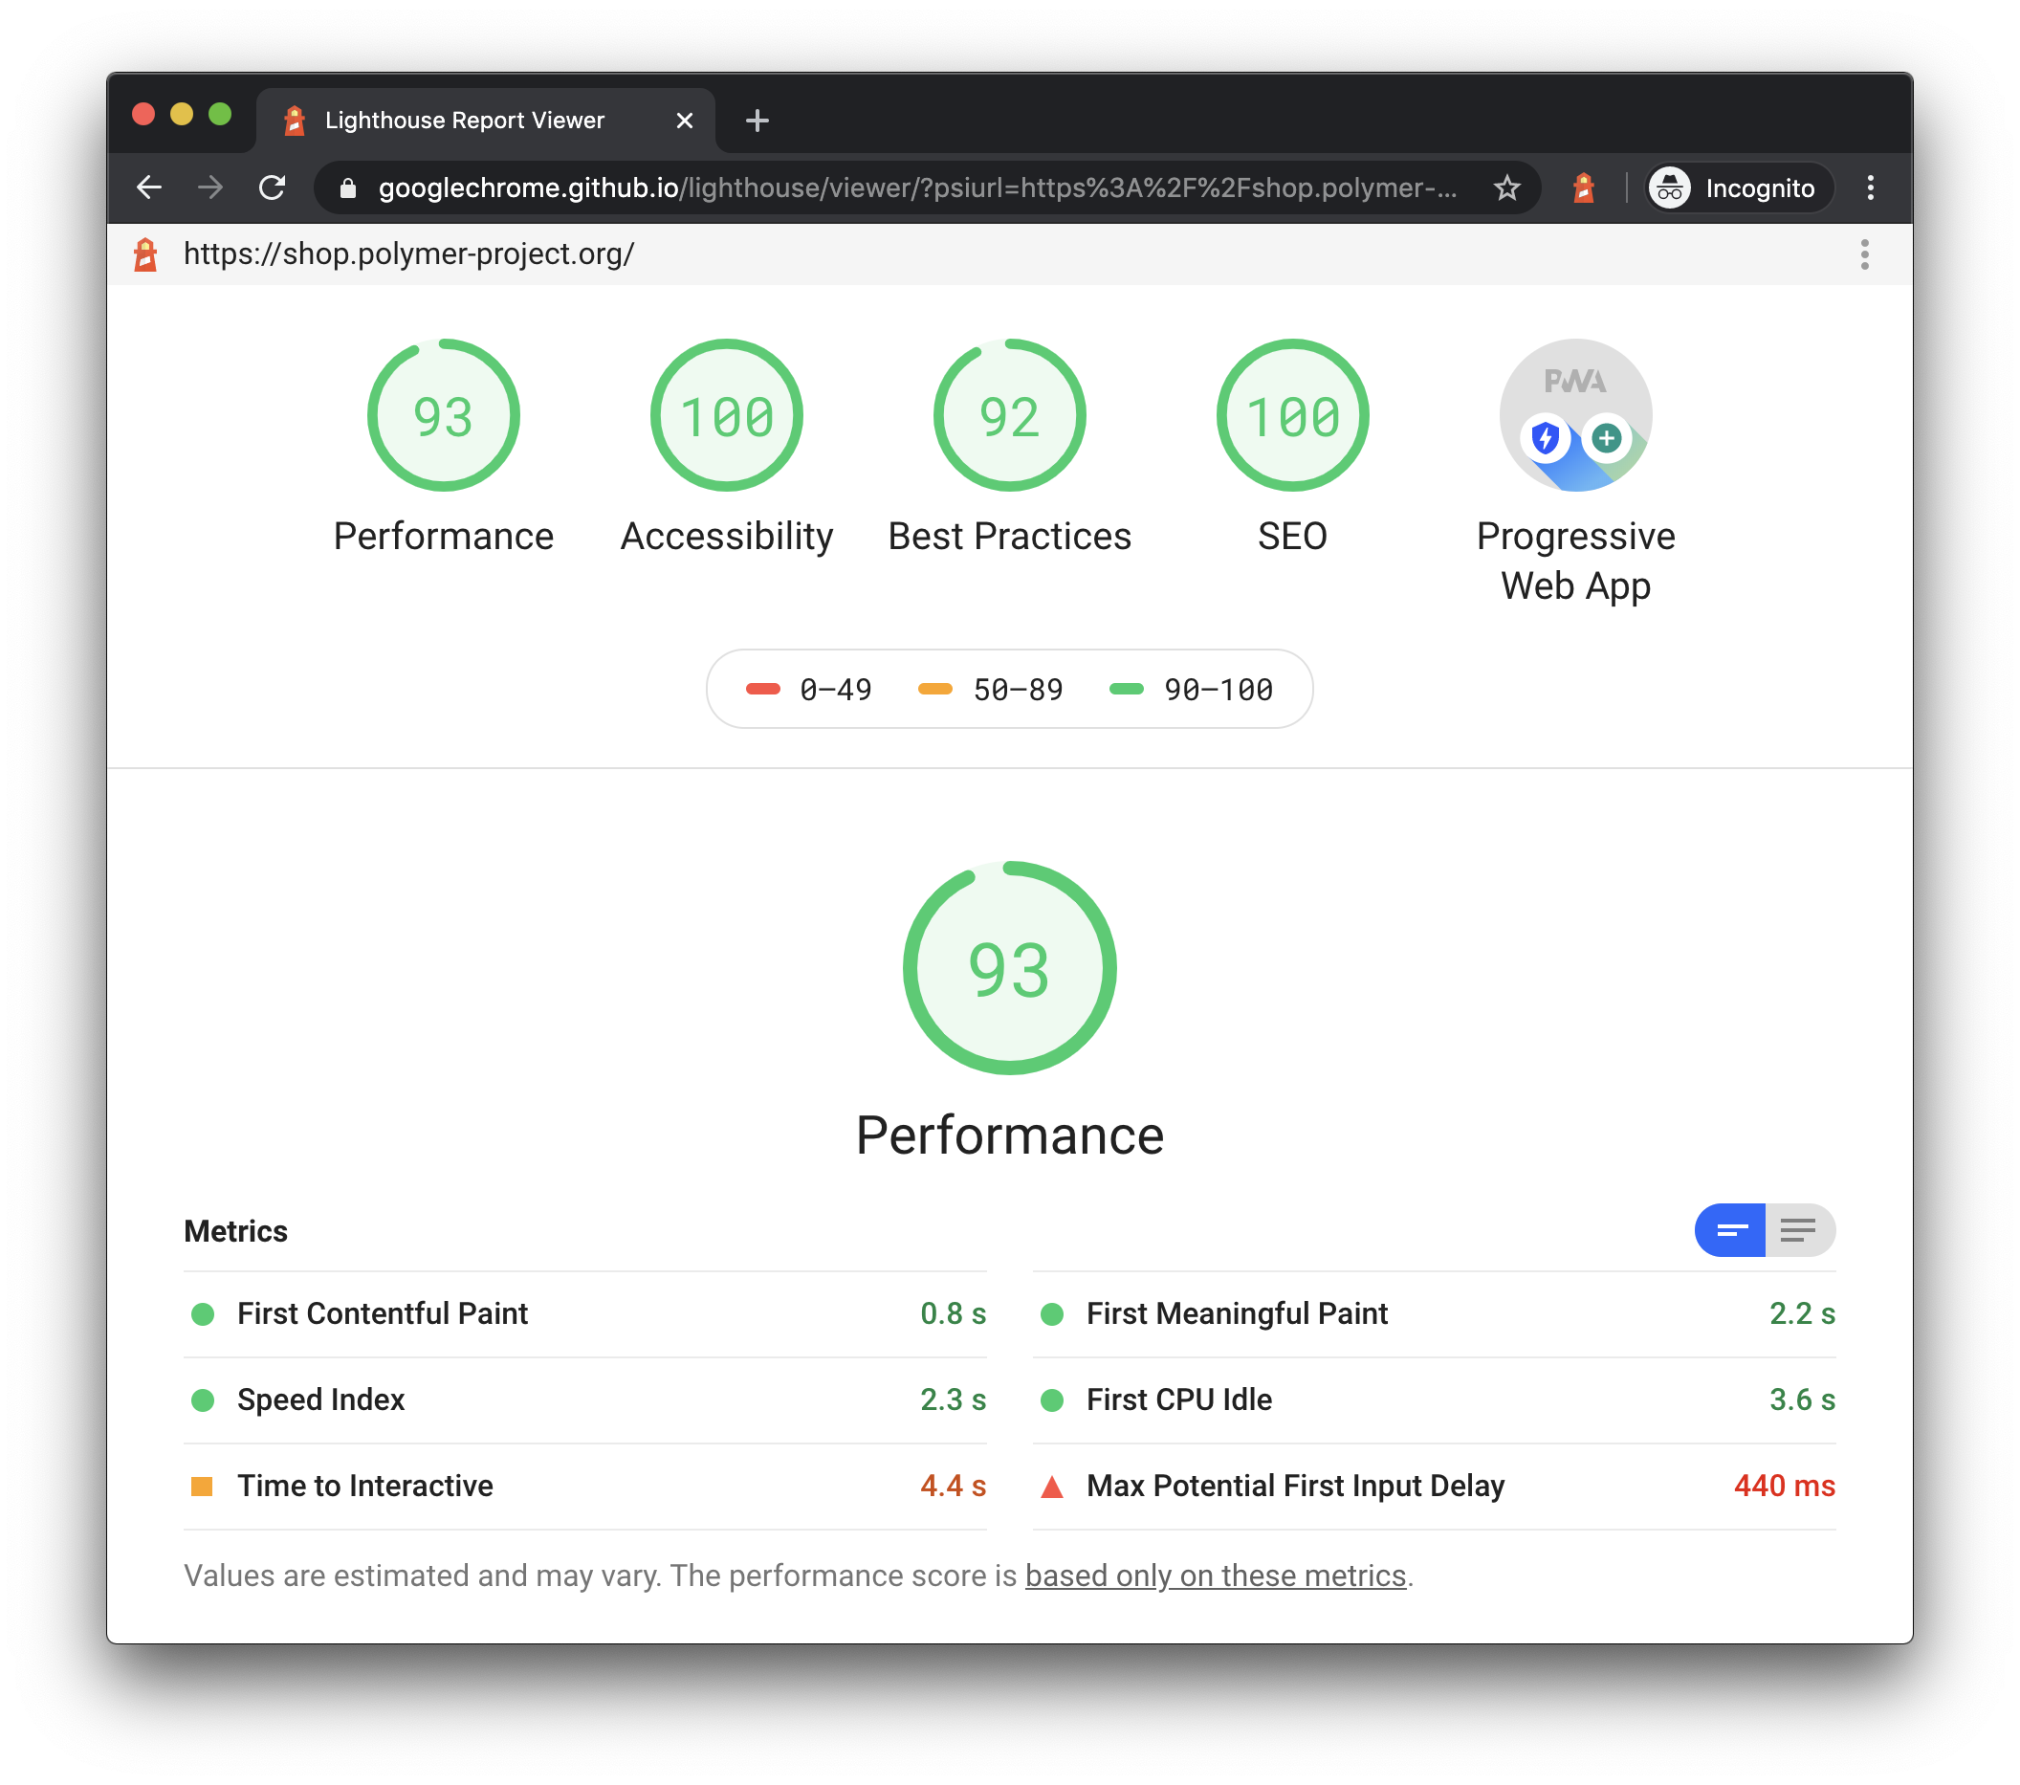
\includegraphics[width=.8\textwidth]{./Figures/Ejemplo de auditoria Lighthouse.png}
	\caption{Ejemplo de auditoría realizada en Lighthouse \protect\footnotemark.}
	\label{fig:ejemploDeAuditoriaLighthouse}
\end{figure}

\footnotetext{Imagen tomada de \url{https://es.semrush.com/blog/como-utilizar-google-lighthouse/}}

La elección de Lighthouse como herramienta de auditorías es debida a su integración incorporada en el navegador y sus pruebas extensivas en diferentes áreas. Otro factor influyente en la decisión fue que además de dar un amplio diagnóstico, también brinda posibles soluciones para cada uno de los problemas encontrados.
